\subsubsection{High current behavior}\label{sssec:high_current_behavior}
In this section the $20\,M\Omega$ input resistor is replaecd with a $4\,M\Omega$ resistor. The main goal is to observe the ROIC for very large currents.


\Cref{fig:bre_slopes} shows the same plot as \cref{fig:slopes}, but this time with larger currents. Where a minimum slope could be observed at \cref{fig:slopes}, it is more prevalent here. This also shows more information about the behavior of VBO. For small voltages the VBO does not increase, but as the voltages get larger, one can observe that the voltages of VBO start rising when the OUT is done with decharging. It is also interesting to note that VBO seems to be not affected by the minimum slope at OUT. This gives rise to the hypothesis that the OUT is limited by the source follower. 

\begin{figure}[h]
    \centering
    \begin{subfigure}[b]{0.475\textwidth}
        \centering
        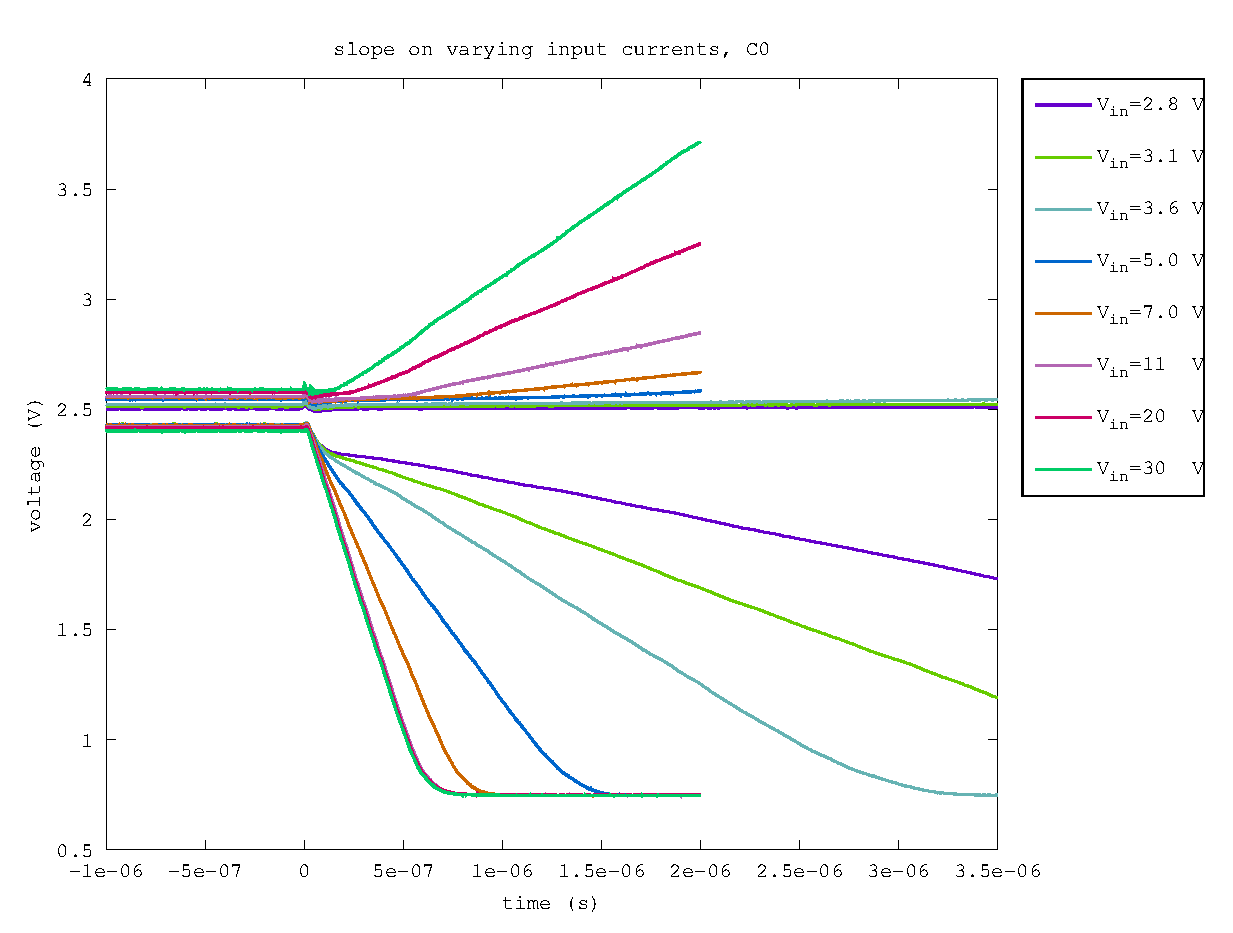
\includegraphics[width=\textwidth]{fig/bre_slope_450fF.eps}
        \caption[Network2]%
        {$C=450\,fF$}    
        \label{fig:bre_slopes_450fF}
    \end{subfigure}
    \hfill
    \begin{subfigure}[b]{0.475\textwidth}  
        \centering 
        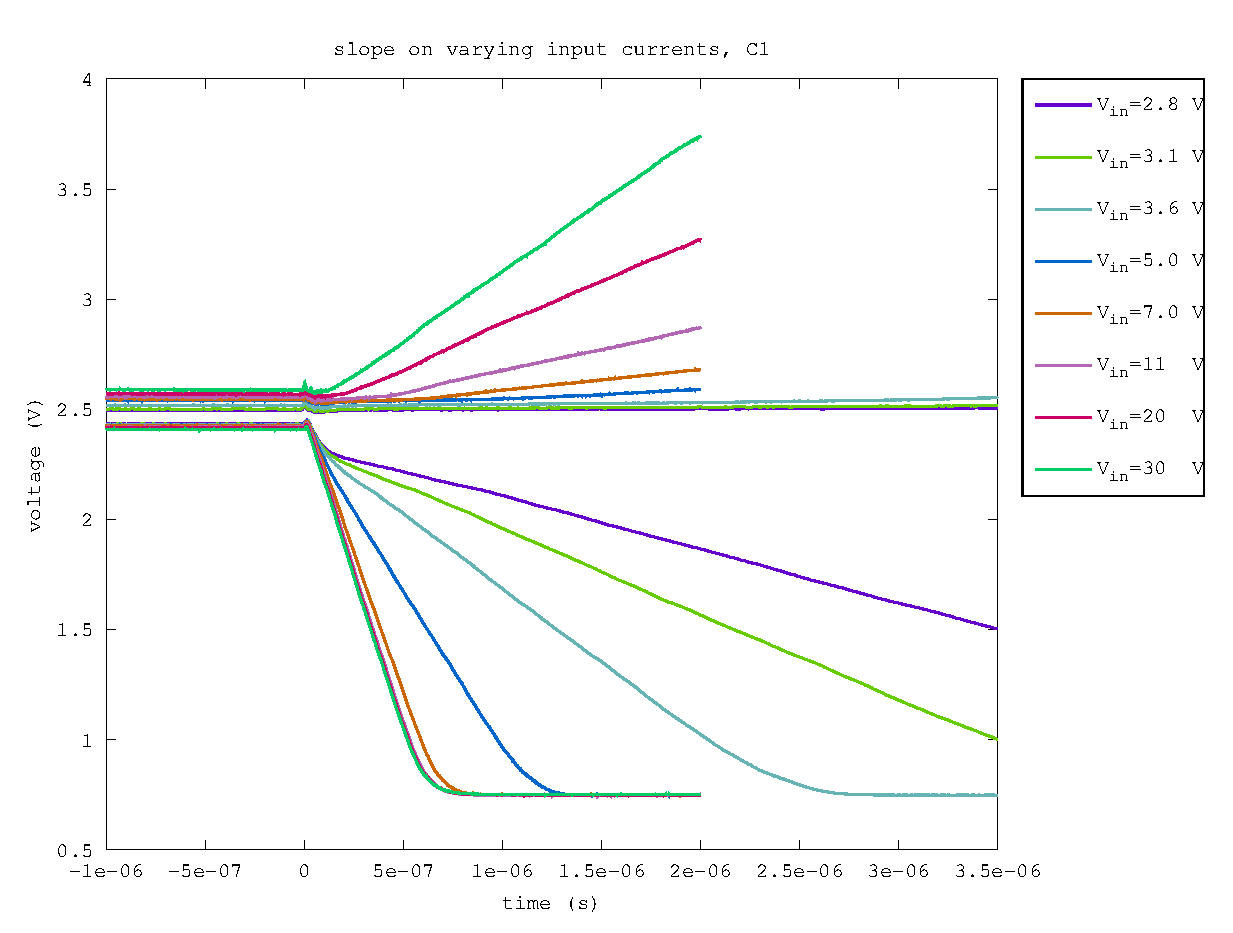
\includegraphics[width=\textwidth]{fig/bre_slope_350fF.eps}
        \caption{$C=350\,fF$}    
        \label{fig:bre_slopes_350fF}
    \end{subfigure}
    \vskip\baselineskip
    \begin{subfigure}[b]{0.475\textwidth}   
        \centering 
        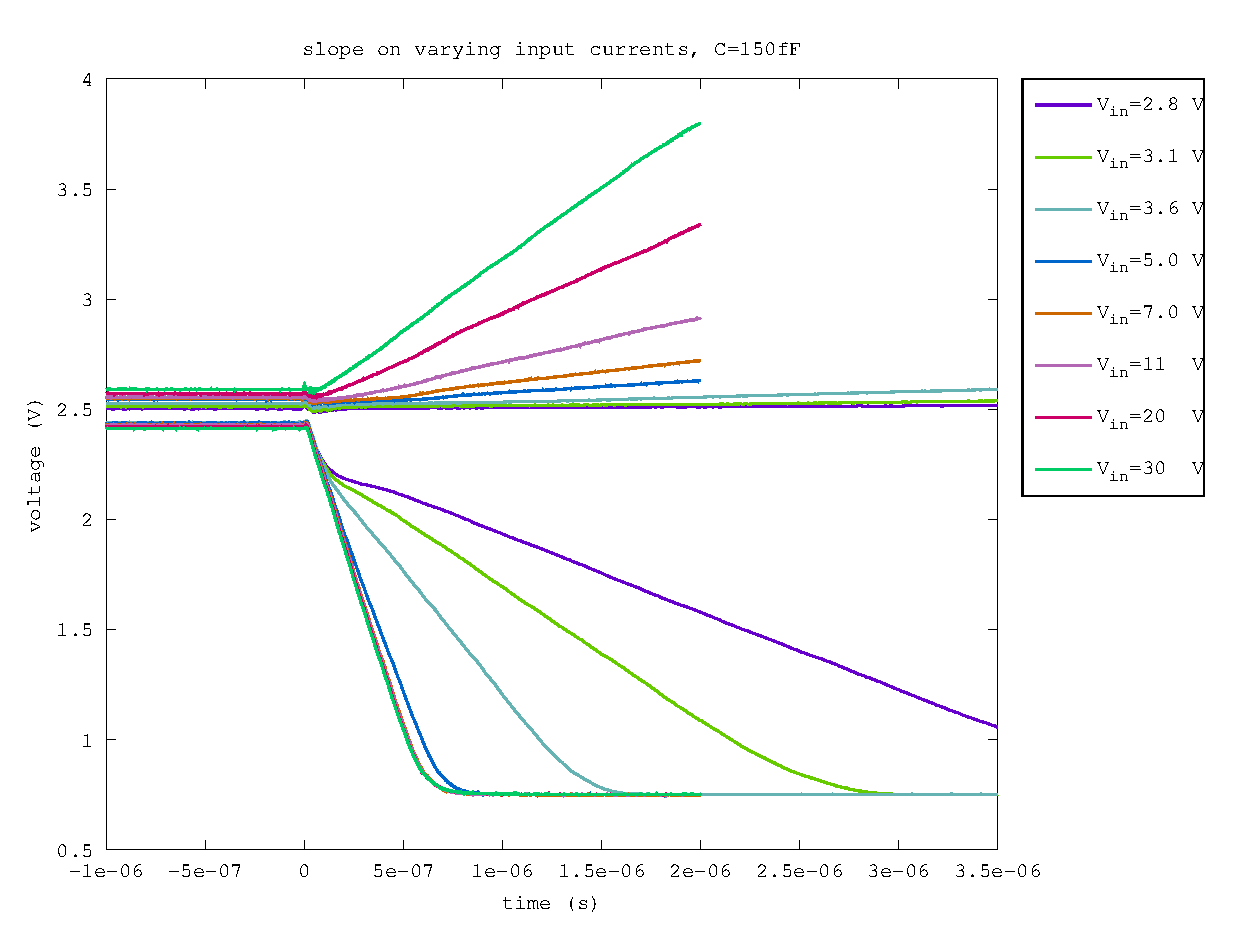
\includegraphics[width=\textwidth]{fig/bre_slope_150fF.eps}
        \caption{$C=150\,fF$}    
        \label{fig:bre_slopes_150fF}
    \end{subfigure}
    \quad
    \begin{subfigure}[b]{0.475\textwidth}   
        \centering 
        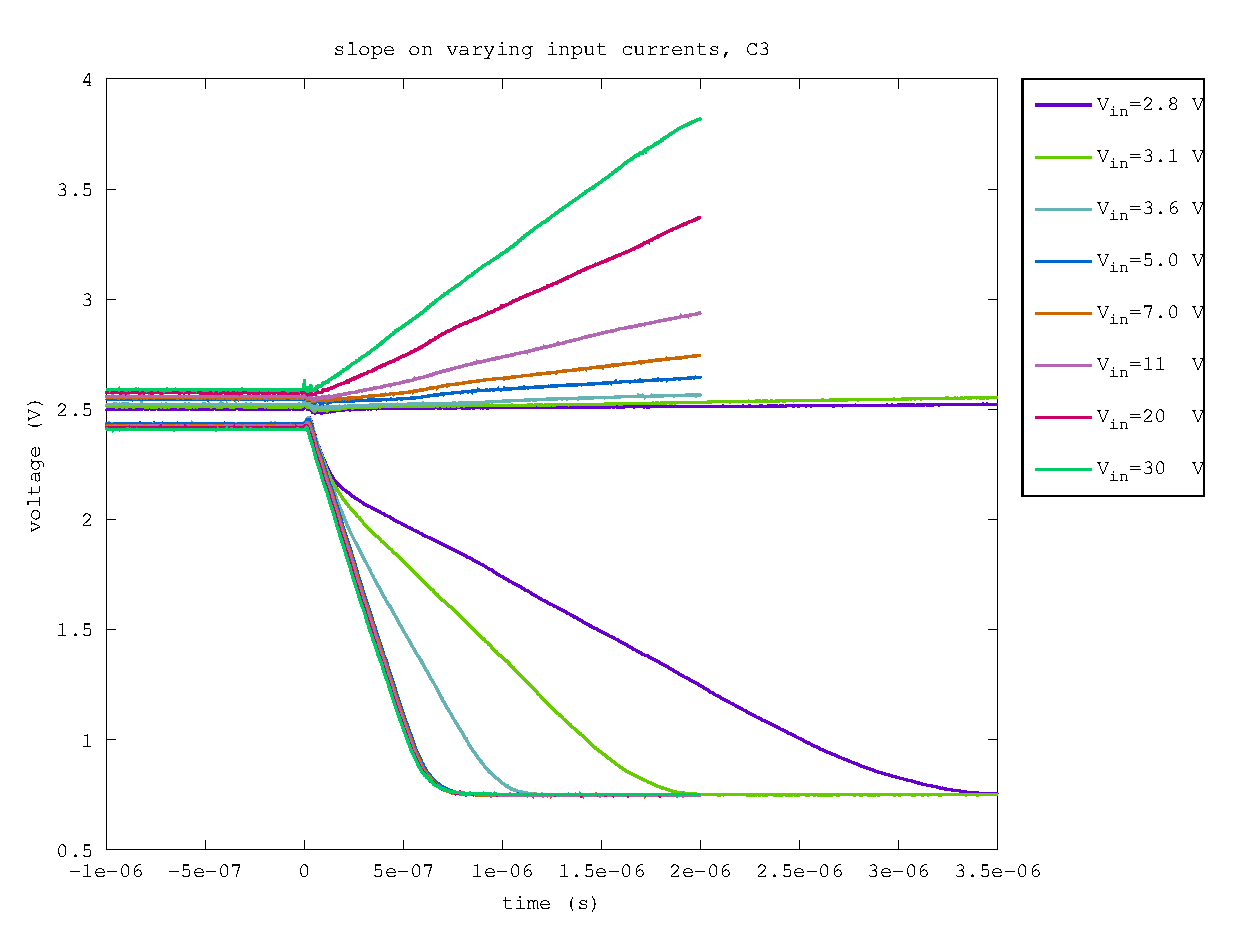
\includegraphics[width=\textwidth]{fig/bre_slope_50fF.eps}
        \caption{$C=50\,fF$}    
        \label{fig:bre_slopes_50fF}
    \end{subfigure}
    \caption{Expected versus measured charge up times for different input voltages. The input voltage is connected to the input through a resistor of $4\,M\Omega$}
    \label{fig:bre_slopes}
\end{figure}

\Cref{fig:bre_charges} shows a similar plot as in \cref{fig:charges} but with higher currents. In \cref{fig:charges} one could observe that all currents fitted to the same line, but deviated at higher currents. This effect is also observed here, but in a stronger form. Which is to be expected.

\begin{figure}[h]
    \centering
    \begin{subfigure}[b]{0.475\textwidth}
        \centering
        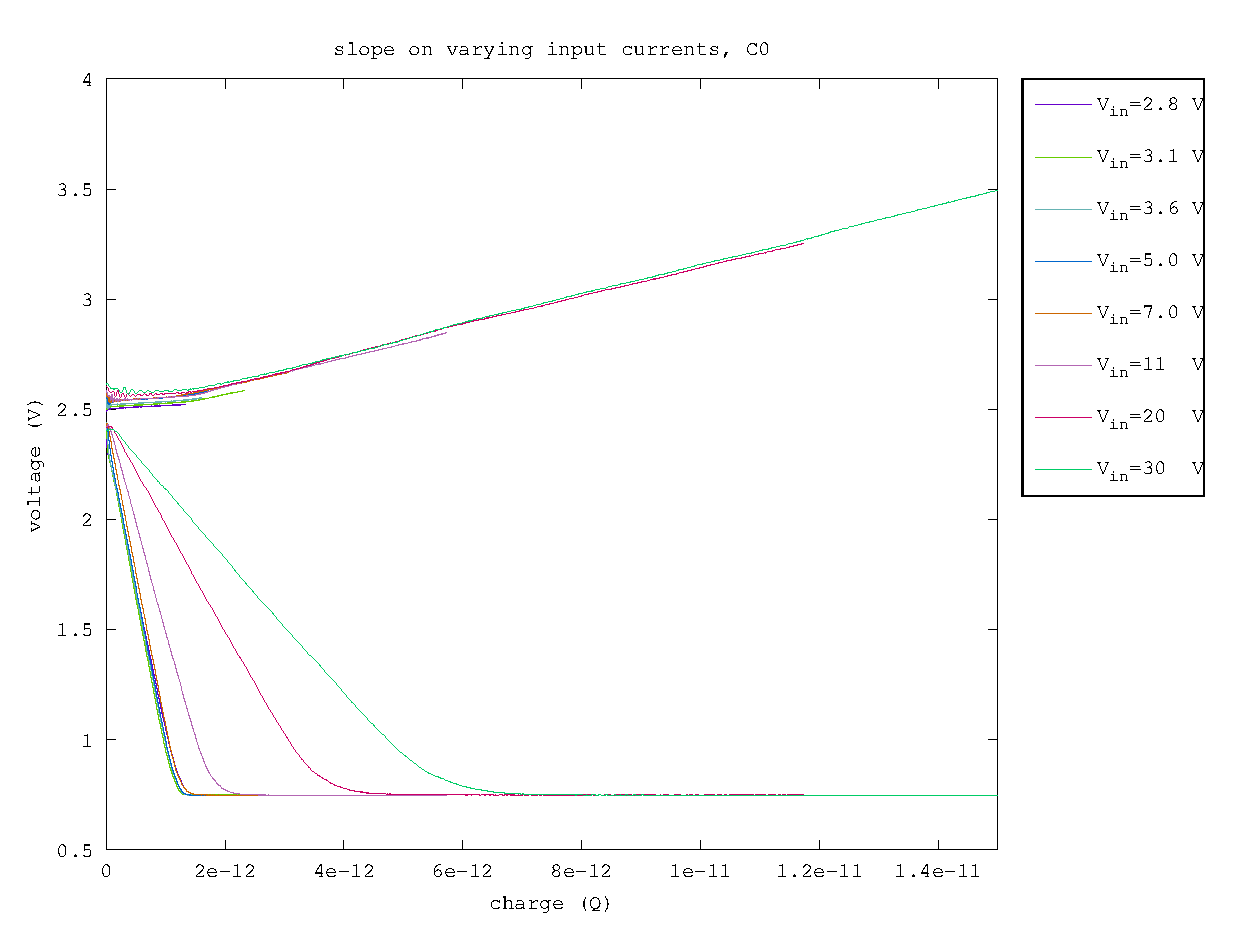
\includegraphics[width=\textwidth]{fig/bre_charge_450fF.eps}
        \caption[Network2]%
        {$C=450\,fF$}    
        \label{fig:bre_charges_450fF}
    \end{subfigure}
    \hfill
    \begin{subfigure}[b]{0.475\textwidth}  
        \centering 
        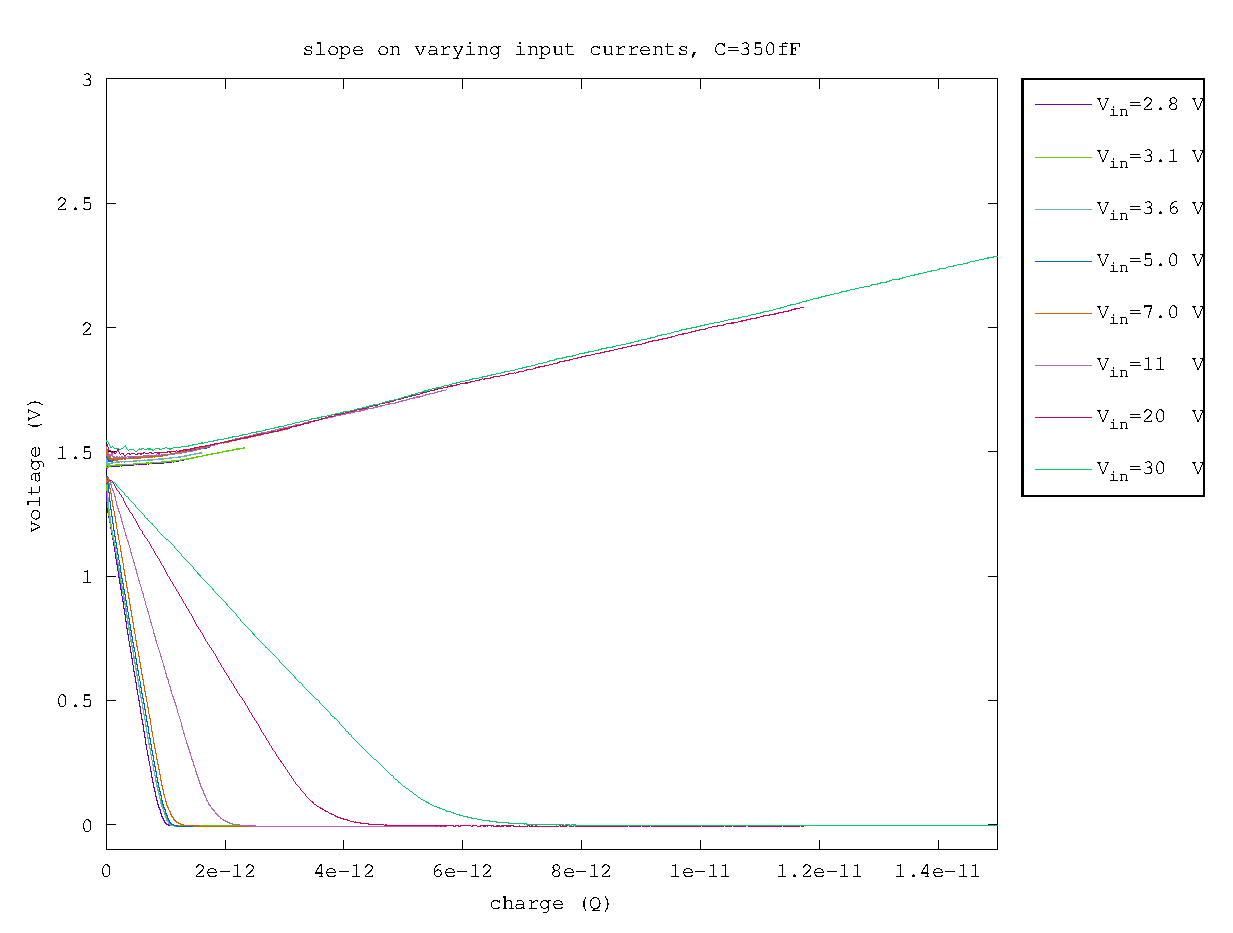
\includegraphics[width=\textwidth]{fig/bre_charge_350fF.eps}
        \caption{$C=350\,fF$}    
        \label{fig:bre_charges_350fF}
    \end{subfigure}
    \vskip\baselineskip
    \begin{subfigure}[b]{0.475\textwidth}   
        \centering 
        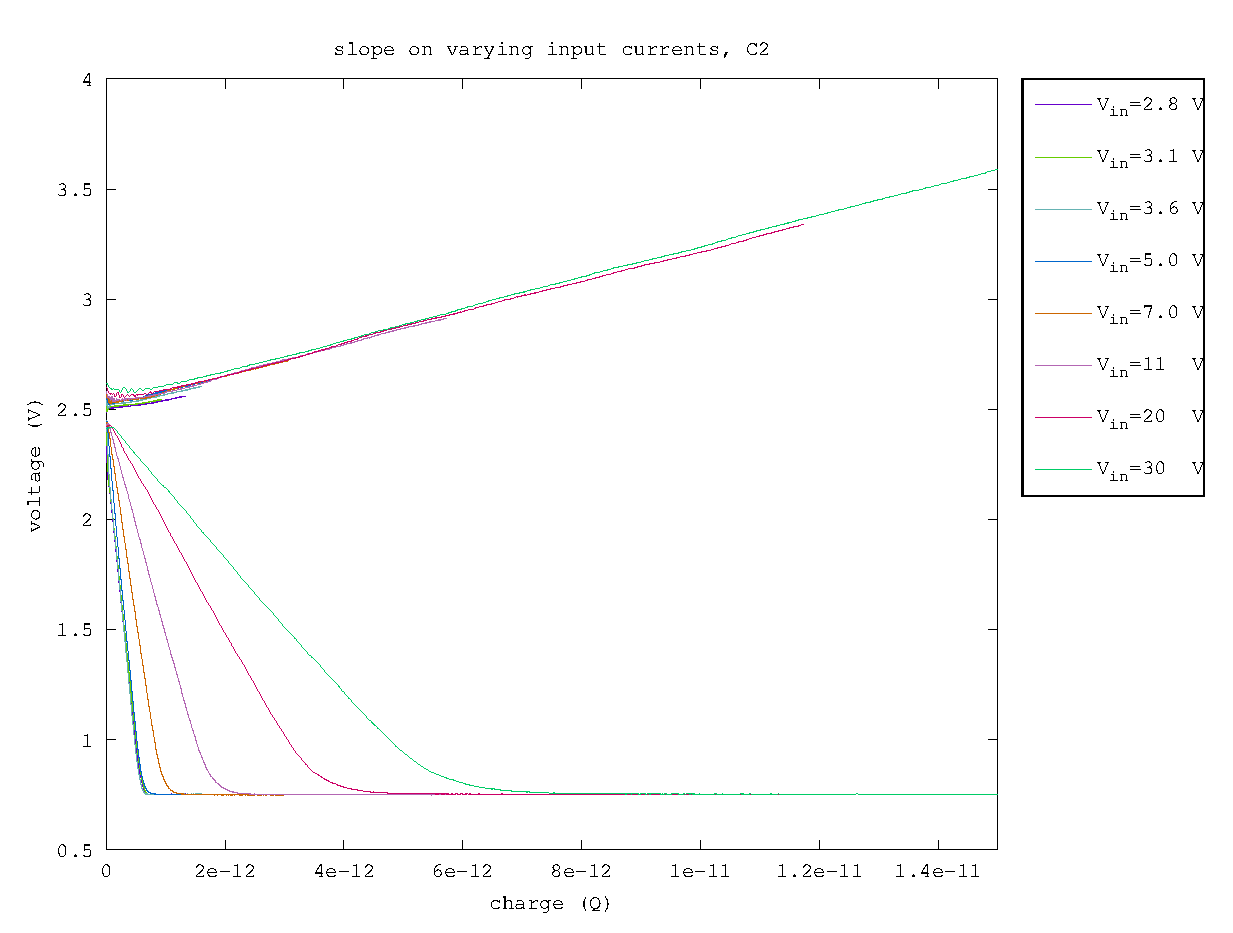
\includegraphics[width=\textwidth]{fig/bre_charge_150fF.eps}
        \caption{$C=150\,fF$}    
        \label{fig:bre_charges_150fF}
    \end{subfigure}
    \quad
    \begin{subfigure}[b]{0.475\textwidth}   
        \centering 
        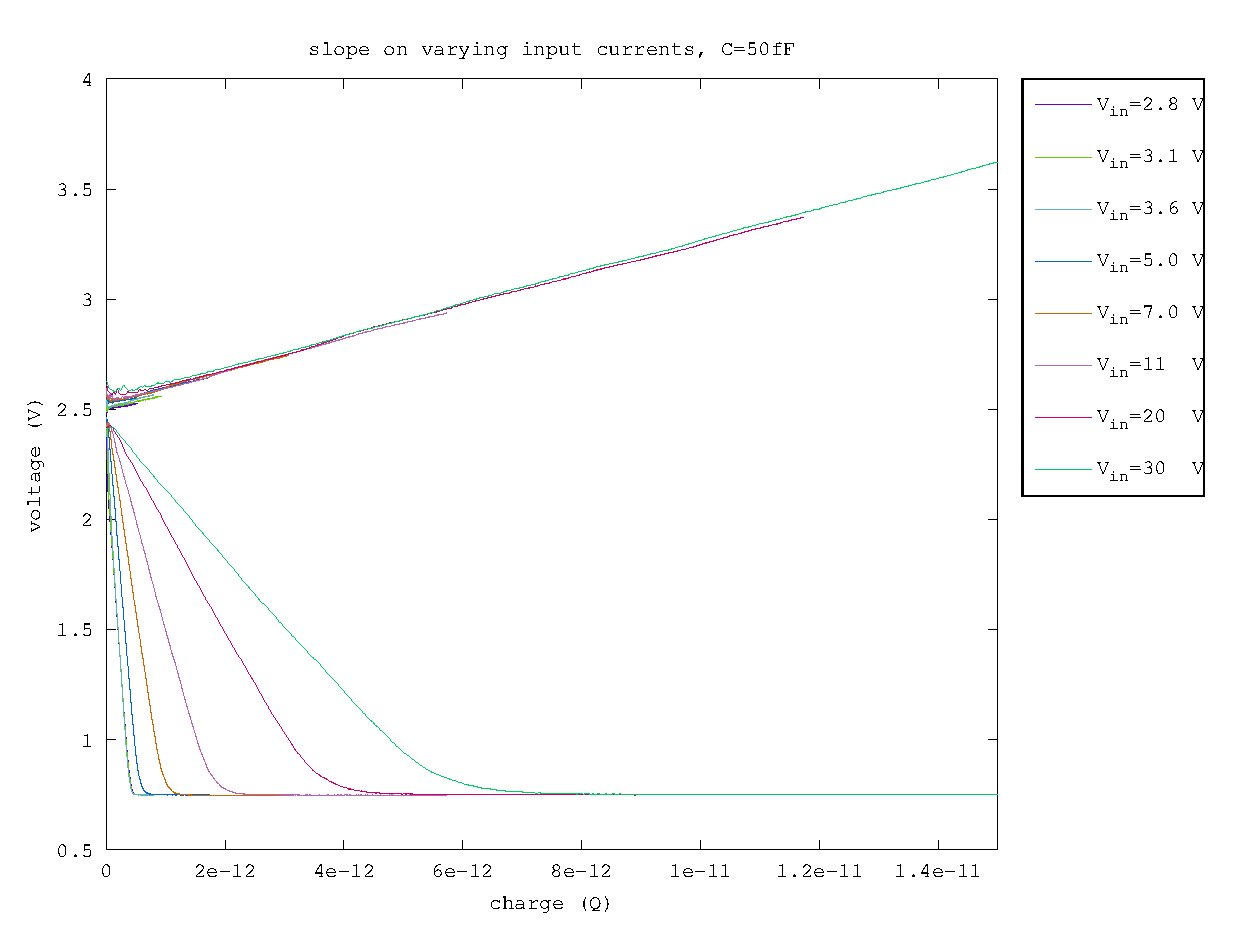
\includegraphics[width=\textwidth]{fig/bre_charge_50fF.eps}
        \caption {$C=50\,fF$}    
        \label{fig:bre_charges_50fF}
    \end{subfigure}
    \caption{This plot is showing charge versus voltage}
    \label{fig:bre_charges}
\end{figure}

\Cref{fig:bre_d_slopes} shows a plot of $\delta V/\delta Q$ against charge. Note that the behavior for the low voltages differ across the different capacitances, but that the high voltages are not affected by a change in capacitance. This observation agrees with the hypothesis that the output is not limited by the input current, but by the speed of the source follower at the output.

\begin{figure}[h]
    \centering
    \begin{subfigure}[b]{0.475\textwidth}
        \centering
        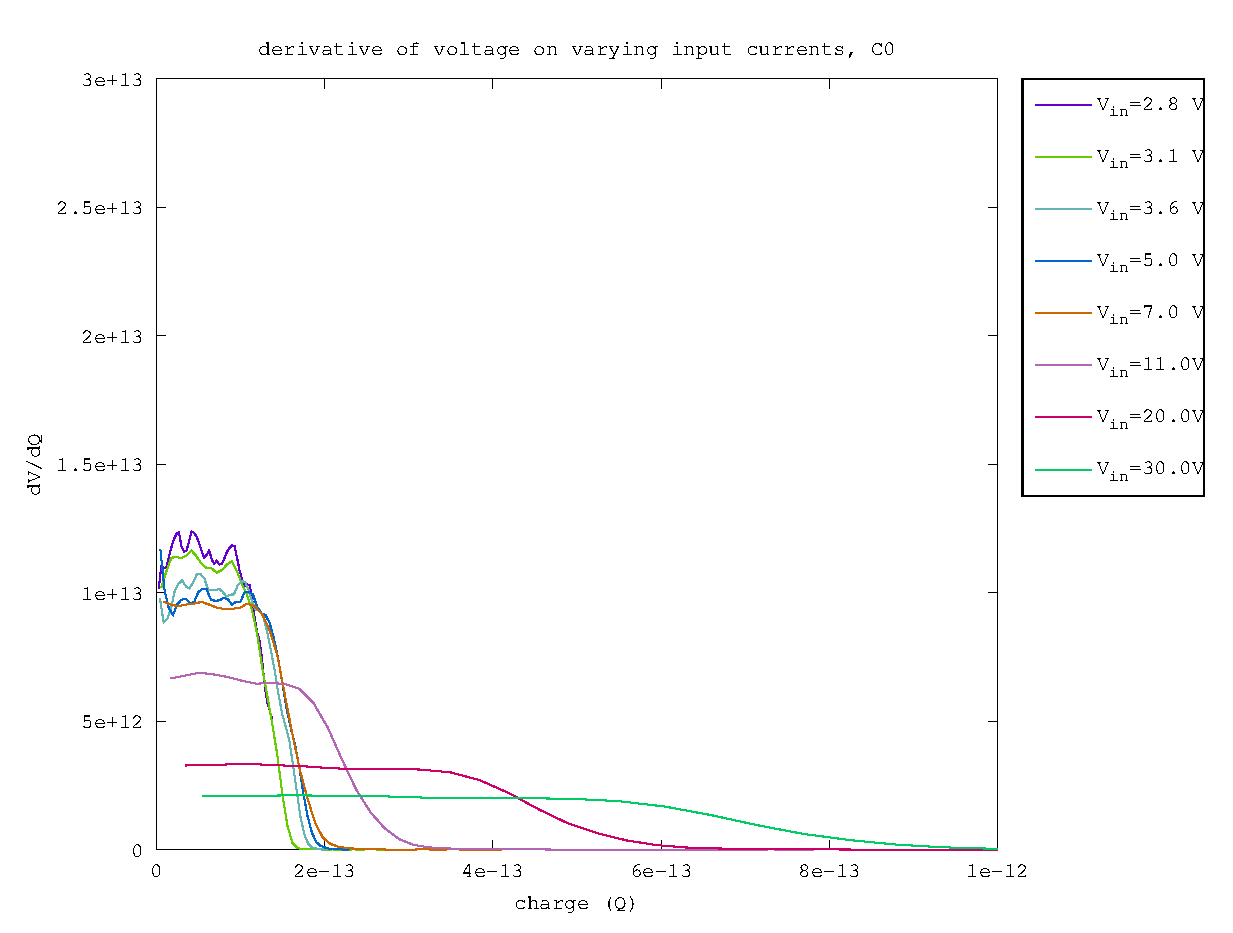
\includegraphics[width=\textwidth]{fig/bre_d_slope_450fF.eps}
        \caption[Network2]%
        {$C=450\,fF$}    
        \label{fig:bre_d_slopes_450fF}
    \end{subfigure}
    \hfill
    \begin{subfigure}[b]{0.475\textwidth}  
        \centering 
        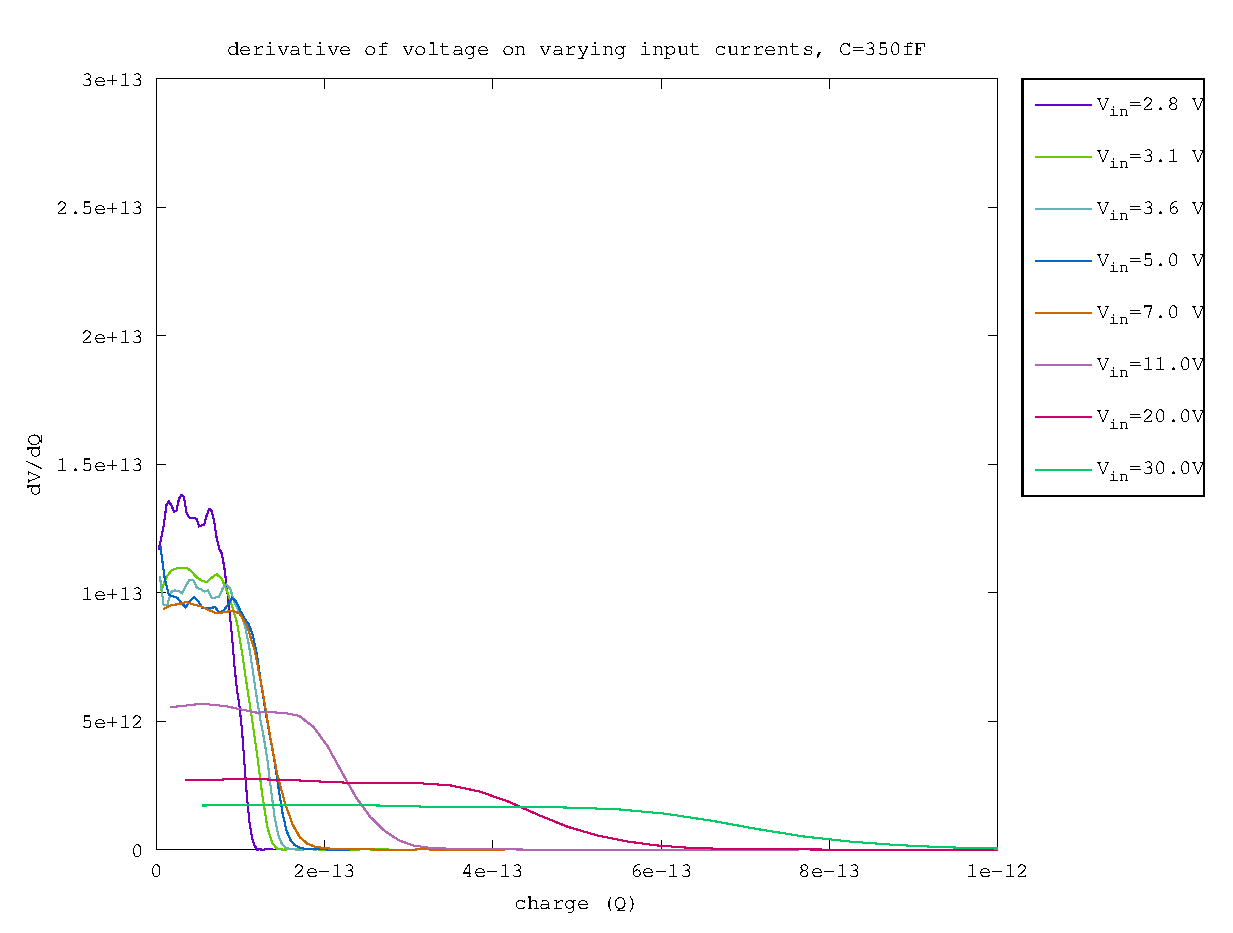
\includegraphics[width=\textwidth]{fig/bre_d_slope_350fF.eps}
        \caption {$C=350\,fF$}    
        \label{fig:bre_d_slopes_350fF}
    \end{subfigure}
    \vskip\baselineskip
    \begin{subfigure}[b]{0.475\textwidth}   
        \centering 
        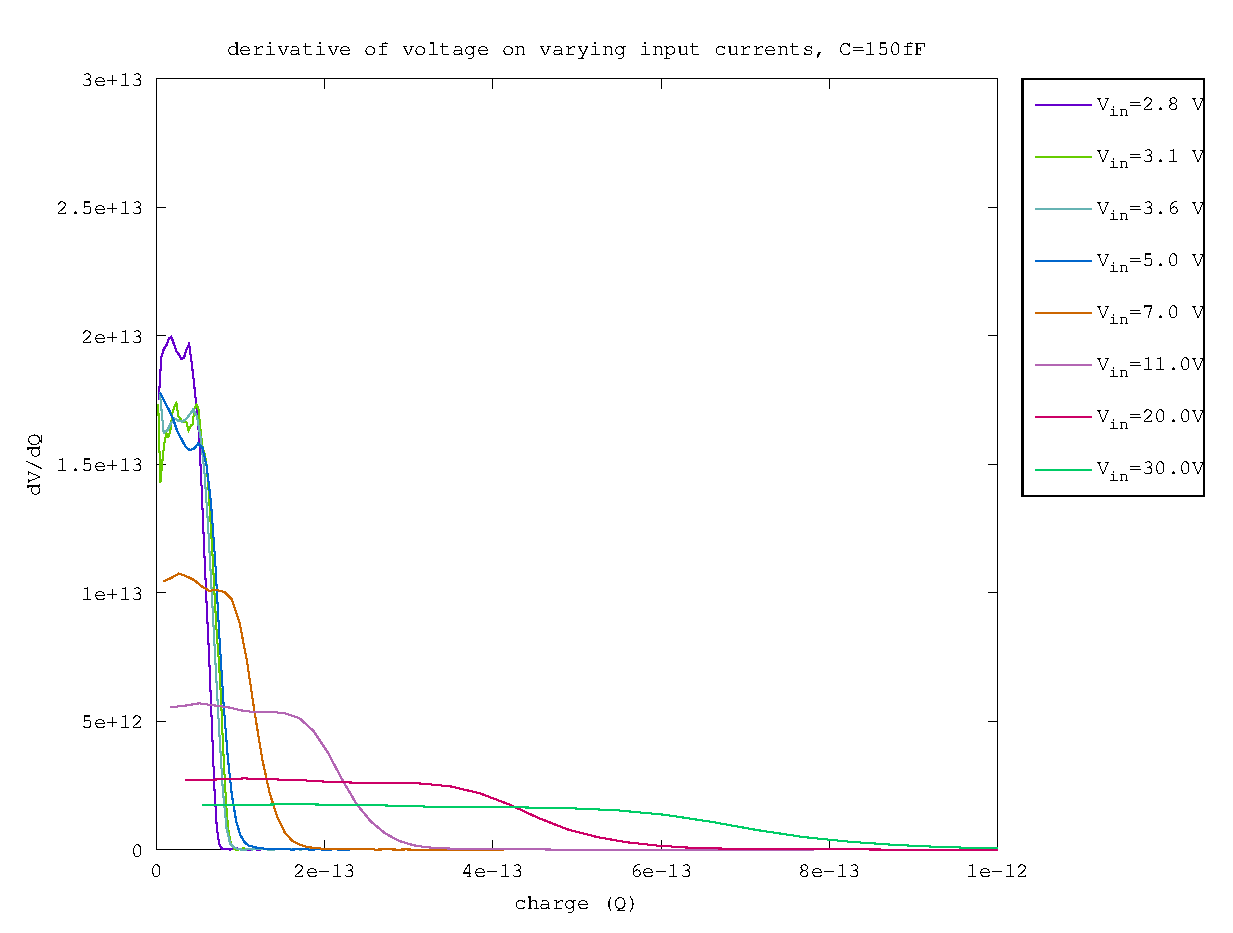
\includegraphics[width=\textwidth]{fig/bre_d_slope_150fF.eps}
        \caption {$C=150\,fF$}    
        \label{fig:bre_d_slopes_150fF}
    \end{subfigure}
    \quad
    \begin{subfigure}[b]{0.475\textwidth}   
        \centering 
        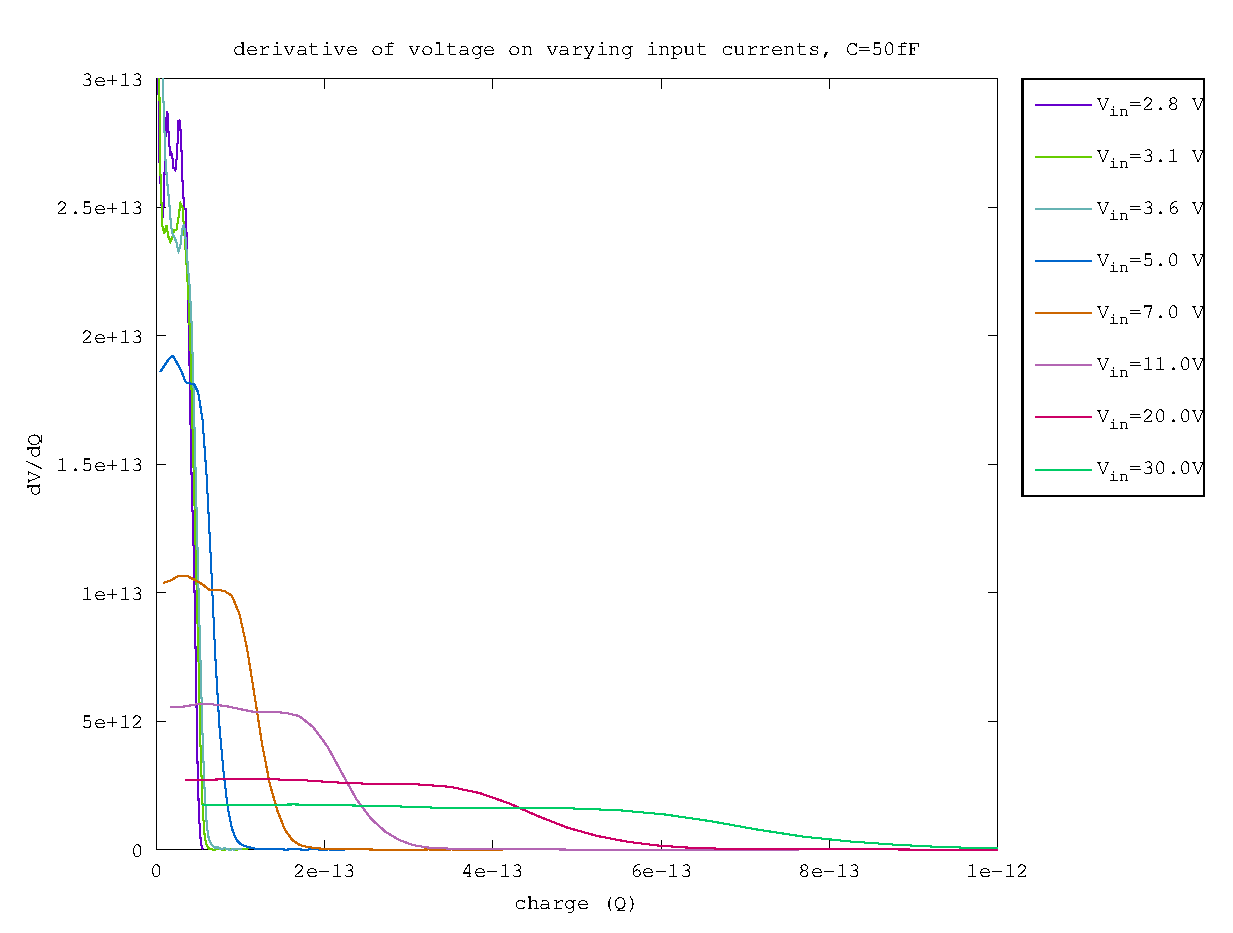
\includegraphics[width=\textwidth]{fig/bre_d_slope_50fF.eps}
        \caption{$C=50\,fF$}    
        \label{fig:bre_d_slopes_50fF}
    \end{subfigure}
    \caption{The plot shows dv/dt against time. The plot is in log scale, which allows for an easy read on the maximum slope and the time needed to discharge the integrator capacitance. }
    \label{fig:bre_d_slopes}
\end{figure}

\Cref{fig:bre_e_vs_m} shows the same plot as \cref{fig:e_vs_m}, but with higher current. This plot clearly shows that all four capacitance configurations saturate at a $\delta V\delta t \approx 3.1\,V$. This cannot be a limit applied to the input, because the capacitances are different. Therefore the output is limiting this, conform previous observations.

\begin{figure}[h]
    \centering
    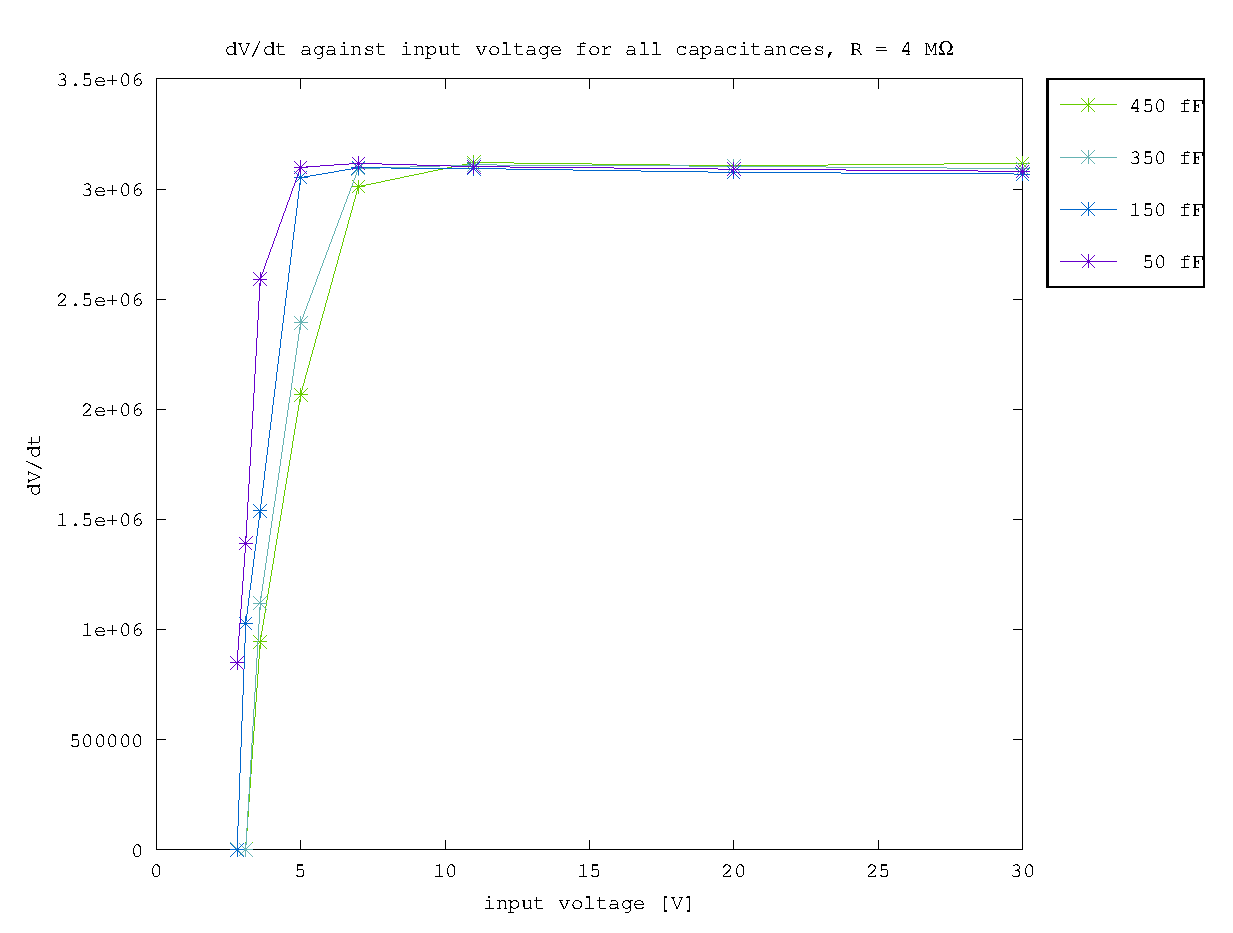
\includegraphics[width=\textwidth]{fig/bre_vin_vs_time_sat.eps}
    \caption {dV/dt against input voltage for all four capacitances. The x indicate the measurements.}    
    \label{fig:bre_e_vs_m}
\end{figure}

\clearpage
